\documentclass[10pt,aspectratio=169]{beamer}

\usetheme[progressbar=frametitle,numbering=fraction]{metropolis}
\usepackage{appendixnumberbeamer}

\usepackage{booktabs}
\usepackage[scale=2]{ccicons}
\usepackage{graphicx}
\usepackage{tabularx}
\graphicspath{{./images/}}

\usepackage{pgfplots}
\usepackage{frcursive}
\usepackage{media9}
%\usepackage{multimedia}
\usepackage[T1]{fontenc}
\usepackage{hyperref}
\usepgfplotslibrary{dateplot}
\usepackage{xspace}
\usepackage{stmaryrd}
\usepackage{animate}
\usepackage{bm}
\usepackage{tcolorbox}
\usepackage[style=authoryear,backend=biber]{biblatex}
%\usepackage{biblatex}
\bibliography{biblio}

% Center Section titles 
    \setbeamertemplate{section page}{
    \begin{center} % add center if missing
    \begin{minipage}{22em}
    \usebeamercolor[fg]{section title}
    \usebeamerfont{section title}
    %\raggedright % comment out raggedright
    \centering % add centering here to center title
    \insertsectionhead\\[-1ex]
    \usebeamertemplate*{progress bar in section page}
    \par
    \ifx\insertsubsectionhead\@empty\else%
    \usebeamercolor[fg]{subsection title}%
    \usebeamerfont{subsection title}%
    \insertsubsectionhead
    \fi
    \end{minipage}
    \end{center}
    \par
    \vspace{\baselineskip}
    }
    

%%%%%%%%%%%%%%%%%%%%%%%%%%%%%%%%%%%%%%%%%%%%%%%%%%%%%%%%%%%%%%%%%%%%%%%%%%%%%%%
% \embedvideo{<poster or text>}{<video file (MP4+H264)>}
%%%%%%%%%%%%%%%%%%%%%%%%%%%%%%%%%%%%%%%%%%%%%%%%%%%%%%%%%%%%%%%%%%%%%%%%%%%%%%
\usepackage[bigfiles]{pdfbase}
\ExplSyntaxOn
%%begin novalidate
\cs_new:Npn\embedvideo#1#2{
%%end novalidate
  \leavevmode
  \pbs_pdfobj:nnn{}{fstream}{{}{#2}}
  \pbs_pdfobj:nnn{}{dict}{
    /Type/Filespec/F~(#2)/UF~(#2)
    /EF~<</F~\pbs_pdflastobj:>>
  }
  \tl_set:Nx\video{\pbs_pdflastobj:}%
  %
  \pbs_pdfobj:nnn{}{dict}{
    /Type/RichMediaInstance/Subtype/Video
    /Asset~\video
    /Params~<</Binding/Foreground>>
  }
  %
  \pbs_pdfobj:nnn{}{dict}{
    /Type/RichMediaConfiguration/Subtype/Video
    /Instances~[\pbs_pdflastobj:]
  }
  %
  \pbs_pdfobj:nnn{}{dict}{
    /Type/RichMediaContent
    /Assets~<<
      /Names~[(#2)~\video]
    >>
    /Configurations~[\pbs_pdflastobj:]
  }
  \tl_set:Nx\rmcontent{\pbs_pdflastobj:}%
  %
  \pbs_pdfobj:nnn{}{dict}{
    /Activation~<<
      /Condition/XA
      /Presentation~<<
        /Transparent~true
        /Style/Embedded
        /PassContextClick~true
      >>
    >>
    /Deactivation~<</Condition/PC>>
  }
  %
  \hbox_set:Nn\l_tmpa_box{#1}
  \tl_set:Nx\l_box_wd_tl{\dim_use:N\box_wd:N\l_tmpa_box}
  \tl_set:Nx\l_box_ht_tl{\dim_use:N\box_ht:N\l_tmpa_box}
  \tl_set:Nx\l_box_dp_tl{\dim_use:N\box_dp:N\l_tmpa_box}
  \pbs_pdfxform:nnnnn{1}{1}{}{}{\l_tmpa_box}
  %
  \pbs_pdfannot:nnnn{\l_box_wd_tl}{\l_box_ht_tl}{\l_box_dp_tl}{
    /Subtype/RichMedia
    /BS~<</W~0/S/S>>
    /Contents~(embedded~video~file:#2)
    /NM~(rma:#2)
    /AP~<</N~\pbs_pdflastxform:>>
    /RichMediaSettings~\pbs_pdflastobj:
    /RichMediaContent~\rmcontent
  }
  \phantom{#1}
}%
\ExplSyntaxOff
%%%%%%%%%%%%%%%%%%%%%%%%%%%%%%%%%%%%%%%%%%%%%%%%%%%%%%%%%%%%%%%%%%%%%%%%%%%%%%


\newcommand{\themename}{\textbf{\textsc{metropolis}}\xspace}
\newcommand{\setfont}[2]{{\fontfamily{#1}\selectfont #2}}
\newcommand{\grad}{\nabla}


\newcommand{\order}[1]{{\ensuremath{#1^{\mathrm{th}}}}}
\newcommand{\mat}[1]{\mathbf{#1}}
\newcommand{\femb}{h_{\mathrm{emb}}}
\newcommand{\fdet}{f_{\mathrm{det}}}
\newcommand{\fset}{\mathcal{F}}
\newcommand{\fdist}{\rho}
\newcommand{\perr}{P_{\mathrm{err}}}
\newcommand{\fext}{g_{\mathrm{ext}}}
\renewcommand{\vec}[1]{\mathbf{#1}}
\newcommand{\pcover}{P_{\mathcal{X}}}
\newcommand{\xcover}{{\mathcal{X}}}
\newcommand{\imspace}{{\mathcal{I}}}
\newcommand{\keys}{{\mathcal{K}}}
\newcommand{\msgs}{{\mathcal{M}}}
\newcommand{\xstegos}[1]{{\mathcal{Y}^{#1}}}
\newcommand{\zstegos}[1]{{\mathcal{Z}^{#1}}}
\newcommand{\pstego}{P_{\mathcal{Y}}}
\newcommand{\hfset}{\mathcal{F}}

% ADD THESE LINES AFTER LOADING THE metropolis THEME
\setbeamertemplate{title page}[default]
% --------

\definecolor{lightgreen}{HTML}{EBF5E0}  % light green
\definecolor{greentheme}{HTML}{7eb356}  % green
\definecolor{orangetheme}{HTML}{ea9010}  % orange

\setbeamersize{text margin left=1.5cm,text margin right=1.5cm}
\setbeamercolor{structure}{fg=greentheme, bg=orangetheme!40}
\setbeamercolor{alerted text}{fg=greentheme}
%\setbeamercolor{progress bar}{greentheme}
%\setbeamercolor{title separator}{greentheme}
%\setbeamercolor{progress bar in head/foot}{greentheme}
%\setbeamercolor{progress bar in section page}{greentheme}

\DeclareMathOperator*{\argmin}{arg\,min} % thin space, limits underneath in displays
\DeclareMathOperator*{\argmax}{arg\,max}

\title{Digital Image Steganography  \\ Using Adversarial Embedding}
\subtitle{Solène Bernard \\ \small{Ph.D. Defense}}
% \date{\today}
\date{18th October, 2021}
\author{Supervised by Tom\'{a}\v{s} Pevn\'{y}, Patrick Bas and John Klein}
%\institute{IEEE Transactions on Information Forensics and Security, 2020}
% \titlegraphic{\hfill\includegraphics[height=1.5cm]{logo.pdf}}

\titlegraphic{
    
\includegraphics[height=0.08\textwidth]{logocentralelille.png}\quad
    
\includegraphics[height=0.08\textwidth]{logocnrs.png}\quad
    
\includegraphics[height=0.08\textwidth]{logoCRIStAL.png}\quad
    
\includegraphics[height=0.08\textwidth]{logounivlille.png}
} 

% \setbeamertemplate{title page}{
%     \begin{minipage}[c][\paperheight]{\textwidth}
%         \centering
%         \ifx\inserttitlegraphic\@empty\else\usebeamertemplate*{title graphic}\fi
%         \vfill%
%         {
%         %\begin{center}
%         %\centering
%         \ifx\inserttitle\@empty\else\usebeamertemplate*{title}\fi
%         \ifx\insertsubtitle\@empty\else\usebeamertemplate*{subtitle}\fi
%         \ifx\insertdate\@empty\else\usebeamertemplate*{date}\fi
%         %\end{center}
%         }
%         \usebeamertemplate*{title separator}
        
%         \begin{center}
%         
\includegraphics[height=0.08\textwidth]{./images/logocentralelille.png}
%         
\includegraphics[height=0.08\textwidth]{./images/logounivlille.png}\\
%         
\includegraphics[height=0.08\textwidth]{./images/logoCRIStAL.png}
%         
\includegraphics[width=0.08\textwidth]{./images/logocnrs.png} \\ \vspace{1em}
%         \small{Advisors: Patrick Bas, John Klein, Tom{\'a}{\v{s}} Pevn{\`y}}
%         \end{center}


%         \begin{minipage}[t]{\textwidth}
%             \centering
%             \ifx\insertinstitute\@empty\else\usebeamertemplate*{institute}\fi
%         \end{minipage}
%         \vfill
%         \vspace*{1mm}
%     \end{minipage}
% }

\setbeamertemplate{frametitle}[default][center]
%\renewcommand*{\insertframenumber}{\arabic{framenumber}/\inserttotalframenumber}

\begin{document}

\maketitle


\section*{Introduction}


\begin{frame}{Context}

    \begin{center}
        \fbox{\begin{minipage}{24em}

            \setfont{frc}{Dear Bob,

            Would you like to listen my new interpretation of Satie? I just published it on Soundcloud. Please be honest. 

            Cheers,

            Alice
            }
        \end{minipage}}
    \end{center}

\end{frame}



\begin{frame}{Context}
    \begin{figure}[h]
        
\includegraphics[width=0.4\textwidth]{soundcloud_logo_2.png}\\\vspace{2em}
        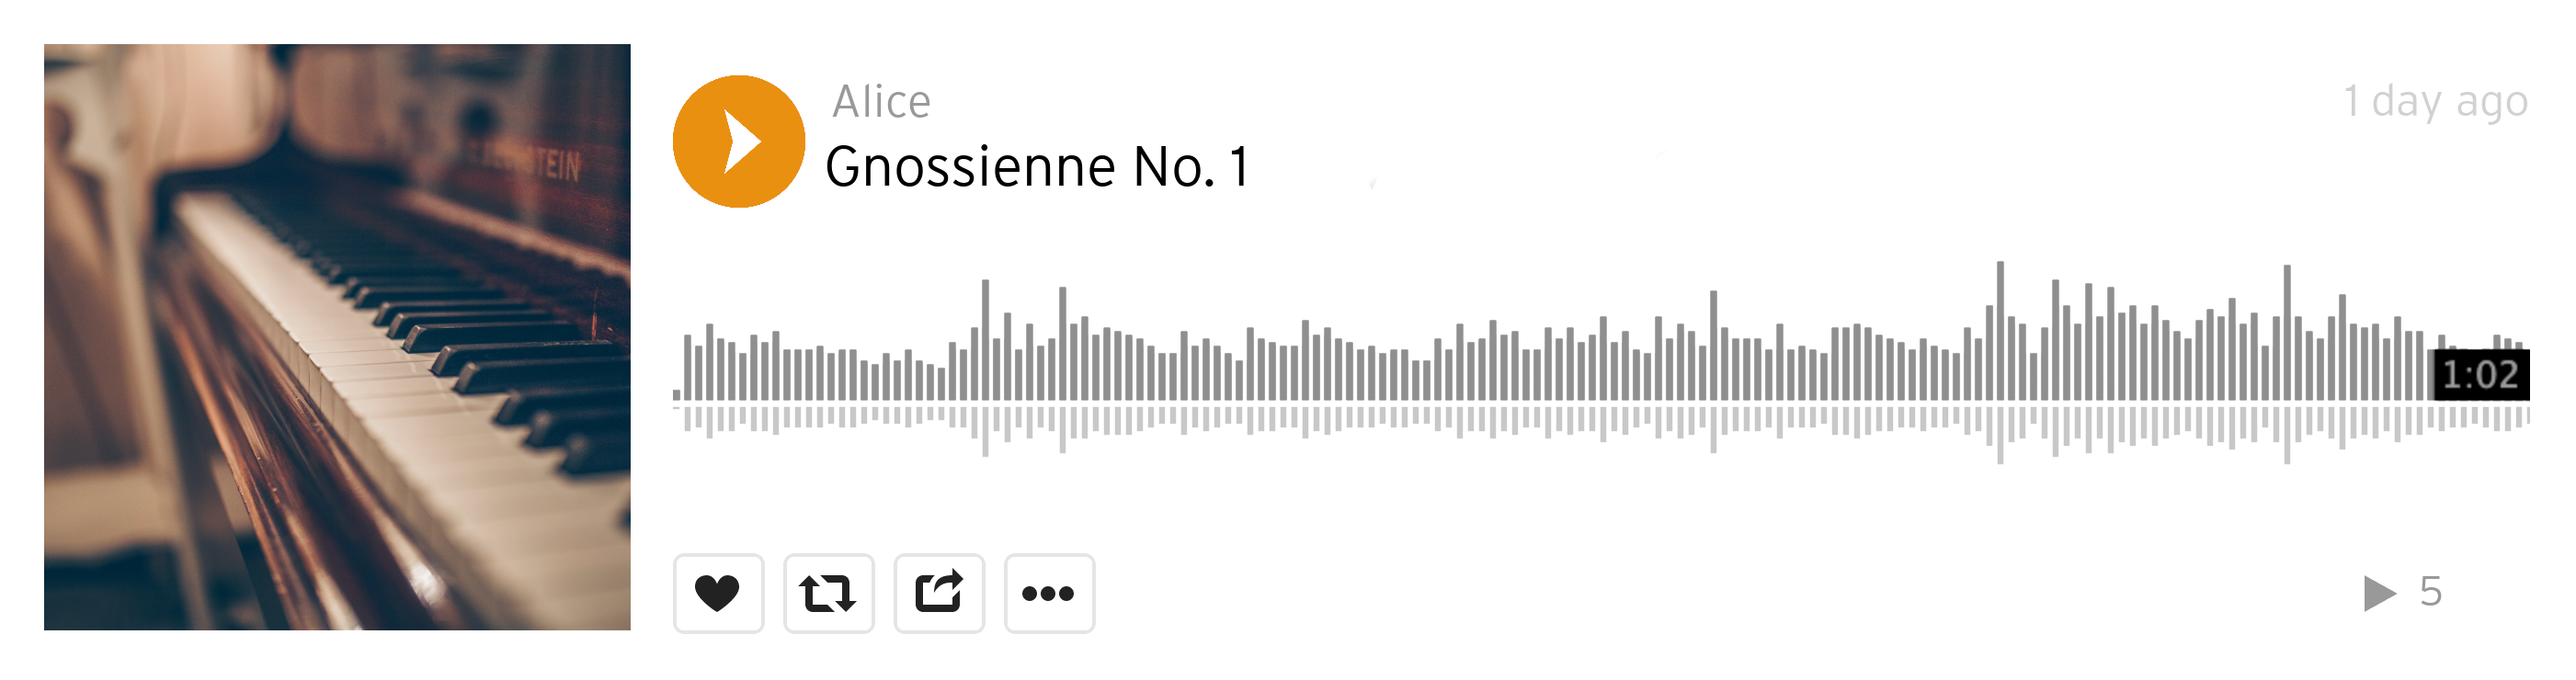
\includegraphics[width=\textwidth]{soundcloud.png}%
        %\includemedia[addresource=stego.mp3,flashvars={source=stego.mp3,&autoPlay=false}]{Play}{APlayer.swf}
    \end{figure}
\end{frame}


% \begin{frame}{Context}
%  \begin{figure}[h]
%     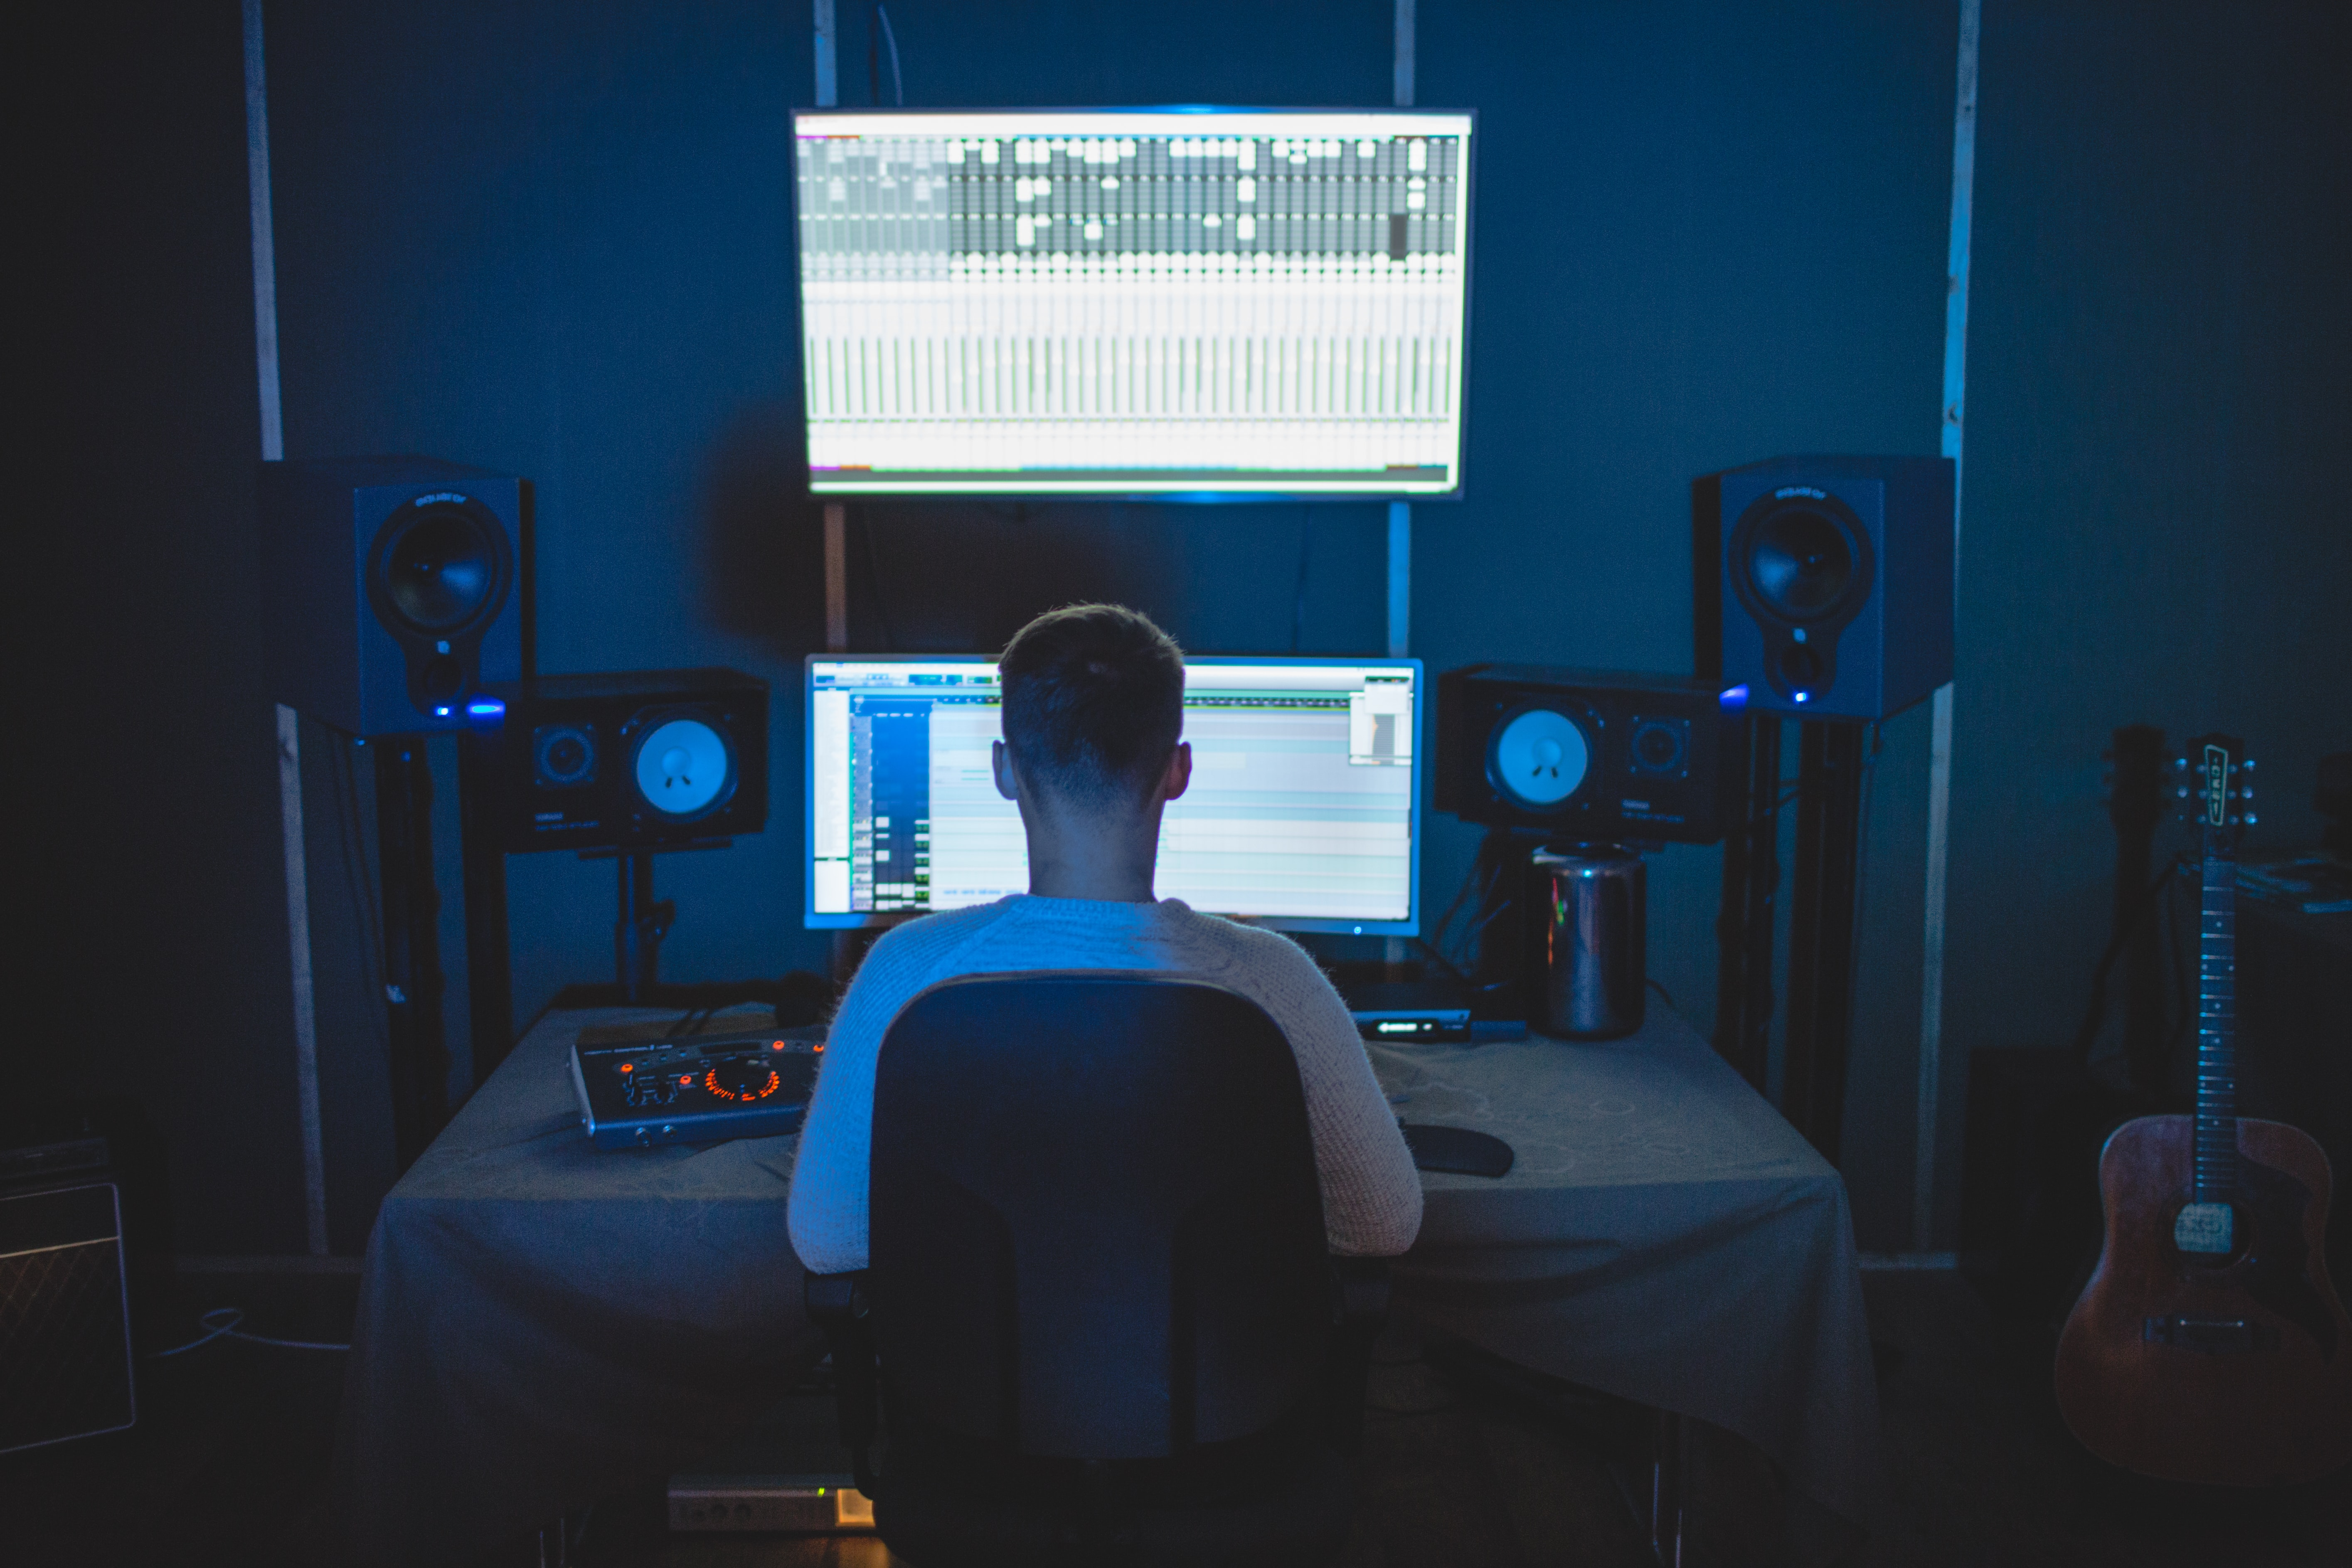
\includegraphics[width=0.9\textwidth]{images/computer.jpg}%
% \end{figure}
% \end{frame}


\begin{frame}{Context}
    %\animategraphics[width=0.9\linewidth]{25}{animation_stego_music/}{0}{29}
    %\includemedia[addresource=stegodecode.mp3,flashvars={source=stegodecode.mp3,&autoPlay=false}]{Play}{APlayer.swf}
\end{frame}


\begin{frame}{Context}

    \begin{figure}[h]
        \only<1>{\includegraphics[height=0.75\textheight]{schema_stego00.pdf}}
        \only<2>{\includegraphics[height=0.75\textheight]{schema_stego01.pdf}}
        \only<3>{\includegraphics[height=0.75\textheight]{schema_stego0.pdf}} 
        \only<4>{\includegraphics[height=0.75\textheight]{schema_stego02.pdf}}
        \only<5>{\includegraphics[height=0.75\textheight]{schema_stego03.pdf}}
        \only<6>{\includegraphics[height=0.75\textheight]{schema_stego.pdf}}
        \only<7>{\includegraphics[height=0.75\textheight]{schema_stego1.pdf}}
        \only<8-9>{\includegraphics[height=0.75\textheight]{schema_stego2.pdf}}
    \end{figure}
    
    \pause \pause \pause \pause \pause \pause \pause \pause
    \centering{\alert{Kerckhoffs’ principle} \\ Eve knows everything about Alice's strategy, except the secret key.}

\end{frame}



\begin{frame}{Modern usage of steganography}
    \begin{itemize}
        \setlength\itemsep{2em}
        \item In some countries the cryptography is prohibited (China, Russia, Colombia, ...) or restricted (France, UK, ...), 
        \item Used by terrorists: an Al Qaeda operative by splicing a video into a copy of the Bruce Willis movie "Die Hard:
        With a Vengeance." (\textit{NY Times, 08/11/2006}),
        \item Used by pedocriminals.
    \end{itemize}
\end{frame}

%\begin{frame}{Context}
%\alert{Kerckhoffs’s principle}

%Eve knows everything about Alice's strategy, except the secret key.

%"Worst-case scenario".
%\end{frame}

\section*{Steganography with digital images}

\begin{frame}{Digital grayscale image structure: Spatial or JPEG}

    \begin{figure}[h]
        \includegraphics[width=0.8\linewidth]{image_structure.pdf}
    \end{figure}

    % \begin{center}
    %         \begin{tabular}{m{5cm} m{5cm}}
    %              Pixels & DCT coefficients
    %         \end{tabular}
    % \end{center}

\end{frame}


\begin{frame}{The first digital images steganographic scheme: LSB replacement}

    Steganography concept: cover modification. 
    \alert{LSB} = "\alert{L}east \alert{S}ignificant \alert{B}it"
    \begin{figure}[h]
        \includegraphics[width=\linewidth]{lsbreplacement2.pdf}
    \end{figure}
    \pause
    At most $+1$ or $-1$ modifications made to the cover image.
\end{frame}

\begin{frame}{The importance of adaptability to the cover image}
    Presence of strong \alert{statistical features} in \textit{natural} images.
    \begin{figure}[h]
        \only<1>{\includegraphics[width=\linewidth]{estonie_LSB.pdf}}
        \only<2>{\includegraphics[width=\linewidth]{estonie_random.pdf}}
    \end{figure}
\end{frame}

\begin{frame}{Adaptative steganography: cost of modification}
    Goal: preserving the image statistics by adapting the embedding to the cover image. 
    \begin{figure}[h]
        \includegraphics[width=0.7\linewidth]{cost.pdf}
    \end{figure}
\end{frame}


\begin{frame}{Adaptative steganography: cost of modification}

    Computation of costs via \alert{heuristic principles}. 
    
    %Example:
    \begin{tabular}{p{0.5\linewidth}p{0.5\linewidth}}
        %\begin{itemize}
            In the spatial domain:
                \begin{itemize}
                    \item S-UNIWARD~\footfullcite{juni},
                    \item HILL~\footfullcite{hill}: 
                        \begin{equation*}
                            \rho=\frac{1}{|\mathbf{x} \star H| \star L_1} \star L_{2}
                        \end{equation*}
                \end{itemize}
            & In the JPEG domain:
                \begin{itemize}
                    %\item HUGO~\footfullcite{hugo}
                    \item J-UNIWARD~\footfullcite{juni},
                    \item UERD~\footfullcite{uerd}.
                \end{itemize}
            
        %\end{itemize}
    \end{tabular}

\end{frame}




\begin{frame}{Adaptative steganography: cost of modification}
    \begin{figure}[h]
        \includegraphics[width=\linewidth]{estoniecostmap.pdf}
    \end{figure}
\end{frame}

\begin{frame}{Alice's objective: embedding while minimizing the distortion}
    \begin{tcolorbox}[colback=lightgreen,colframe=greentheme,title=\textbf{Definition} (Distortion)]
        For an additive cost map $\{\rho_i^b\}$, the  distortion $D$ between the cover $\vec{x}$ and the stego $\vec{y}$ is equal to:
        \begin{equation}
            %D(\mathbf{x},\mathbf{y}) = \sum_{i,b\in\{-1,0,1\}} \rho_i^{b} [y_i - x_i = b]
            D(\mathbf{x},\mathbf{y}) = \sum_{i} \rho_i^{[y_i-x_i]} 
        \end{equation}
    \end{tcolorbox}
\end{frame}

\begin{frame}{Hiding a message with matrix embedding}
    % \begin{figure}[h]
    %     \includegraphics[height=0.2\textheight]{sharedHmatrix.pdf}
    %     \includegraphics[height=0.5\textheight]{formulaSTC.pdf}
    % \end{figure}
    \begin{center}
        \begin{tikzpicture}
            \node (img1) {\includegraphics[height=0.55\textheight]{formulaSTC.pdf}};
            \pause
            \node (img2) at (img1.west)
            {\includegraphics[height=0.3\textheight]{sharedHmatrix.pdf}};
        \end{tikzpicture}
    \end{center}

    \only<3-4>{Algorithm Syndrome-Trellis Code (STC)\footfullcite{filler2011minimizing}  achieves nearly optimal coding.}
    \only<4>{\alert{Bottleneck: costly.}}
\end{frame}


% \begin{frame}{Hiding a message with matrix embedding}
% \begin{figure}[h]
% \includegraphics[width=0.6\linewidth]{images/matrixembedding_4.pdf}
% \end{figure}
% \begin{equation*}
%     D = 5\times \textcolor{greentheme}{1} +  3\times \textcolor{greentheme}{1} + 1\times \textcolor{greentheme}{1} +  2 \times \textcolor{greentheme}{0} + 4 \times \textcolor{greentheme}{1} +  3 \times \textcolor{greentheme}{0} = 13
% \end{equation*}
% \end{frame}


% \begin{frame}{Hiding a message with matrix embedding}
% \begin{figure}[h]
% \includegraphics[width=0.6\linewidth]{images/matrixembedding_2.pdf}
% \end{figure}
% \begin{equation*}
%     D = 5\times \textcolor{greentheme}{0} +  3\times  \textcolor{greentheme}{1} + 1\times \textcolor{greentheme}{1} +  2 \times \textcolor{greentheme}{0} + 4 \times \textcolor{greentheme}{1} +  3 \times \textcolor{greentheme}{0} = 8
% \end{equation*}
% \end{frame}

% \begin{frame}{Hiding a message with matrix embedding}
% \begin{figure}[h]
% \includegraphics[width=0.6\linewidth]{images/matrixembedding_3.pdf}
% \end{figure}
% \begin{equation*}
%     D = 5\times \textcolor{greentheme}{1} +  3\times \textcolor{greentheme}{1} + 1\times \textcolor{greentheme}{0} +  2 \times \textcolor{greentheme}{0} + 4 \times \textcolor{greentheme}{0} +  3 \times \textcolor{greentheme}{0} = 8
% \end{equation*}
% \end{frame}


% \begin{frame}{Hiding a message with matrix embedding}
% \begin{figure}[h]
% \includegraphics[width=0.6\linewidth]{images/matrixembedding_1.pdf}
% \end{figure}
% \begin{equation*}
%     D = 5\times \textcolor{greentheme}{0} +  3\times \textcolor{greentheme}{1} + 1\times \textcolor{greentheme}{0}  +  2 \times \textcolor{greentheme}{0} + 4 \times  \textcolor{greentheme}{0} +  3 \times \textcolor{greentheme}{0} = \boxed{3}
% \end{equation*}
% \end{frame}



% \begin{frame}{Embedding a message}

% \begin{tcolorbox}[colback=lightgreen,colframe=greentheme,title=\textbf{Definition} (The Payload-Limited Sender)]
% The Payload-Limited Sender (PLS) attempts to find a distribution $\pi$ that communicates a required payload $|m|$ while minimizing the distortion $D(\mathbf{x},\mathbf{y}) = \sum_i \rho_i^{y_i - x_i}$:
% \begin{equation}
% \begin{array}{cc}
% \operatorname{minimize} & \mathbb{E}_{\pi}[D]=\sum_{\mathbf{y} \in \mathcal{Y}(\mathbf{x})} \pi(\mathbf{y}) D(\mathbf{x}, \mathbf{y}) \\\\
%  \mbox{ subject to } & H(\pi) = -\sum_{\mathbf{y} \in \mathcal{Y}(\mathbf{x})} \pi(\mathbf{y}) \log_{2} \pi(\mathbf{y}) =|m|
% \end{array}
% \end{equation}

% \end{tcolorbox}
% \end{frame}


\begin{frame}{Simulated steganography - The theory}

    Simulation of embedding, with
    \begin{itemize}
        \item an additive cost map $\{\rho_i^b\}$, 
        \item a length of the hypothetical message $|m|$. 
    \end{itemize}

    \pause 
    Categorical distribution of change for each image coefficient:

    \begin{equation}
        \pi_{i}^b = P_i^j\left(\rho_{i}, \lambda\right) = \frac{e^{-\lambda \rho_{i}^{b}}}{\sum_{b^{\prime} \in \{-1,0,+1\}} e^{-\lambda \rho_{i}^{b^{\prime}}}},
    \end{equation}

    \pause
    where $\lambda$ determined from the entropy constraint:

    \begin{equation}
        \operatorname{Entropy}(\{\pi_i^b\}) = H(\{\pi_i^b\}) = |m|,
    \end{equation}

    with $H$ the binary entropy.

\end{frame}


\begin{frame}{Simulated steganography}

    Pipeline from the cover to the simulated stego:

    \begin{equation*}
        \begin{array}{ccccccccc}
            \mathbf{x} & \longrightarrow & \{\rho^b_i\}_i & \longrightarrow & \{\pi_i^b\}_i &   \xrightarrow{\mbox{\footnotesize{draw}}} & \{b_i\}_i &  \longrightarrow & \mathbf{y} = \mathbf{x} + \mathbf{b} \\ \\
            \mbox{\footnotesize{cover}} & & \mbox{\footnotesize{costs}} & & \mbox{\footnotesize{probabilities}} & & \mbox{\footnotesize{changes}} & &  \mbox{\footnotesize{stego}}
        \end{array}
    \end{equation*}

    \begin{figure}[h]
        %\hspace{-3em}
        \centerline{\includegraphics[width=1\linewidth]{estonie_pipeline.pdf}}
    \end{figure}

    %$\mathcal{A}_a = \{\mathcal{Y}\}$ where $\mathcal{Y}$ stegos obtained from cover set $\mathcal{X}$ with cost maps $\mathcal{R}$.

\end{frame}



%\begin{frame}{Detectability map}
%The embedding operation (named HUGO, J-UNIWARD,S-UNIWARD, ...) can be simulated by changing each pixel $i$ by probability $p_i$ given by : 
%\begin{equation}
%    p_i = \frac{\exp(-\lambda \rho_i)}{1+\exp(-\lambda \rho_i)}
%\end{equation}
%where $\lambda>0$ is a constant determined by the constraint of the size of the message $m$ :
%\begin{equation}
%    m = \sum_{i=1}^{i=n} H(p_i)
%\end{equation}
%\end{frame}

%\begin{frame}{Probability map}
%    \begin{figure}[h]
%        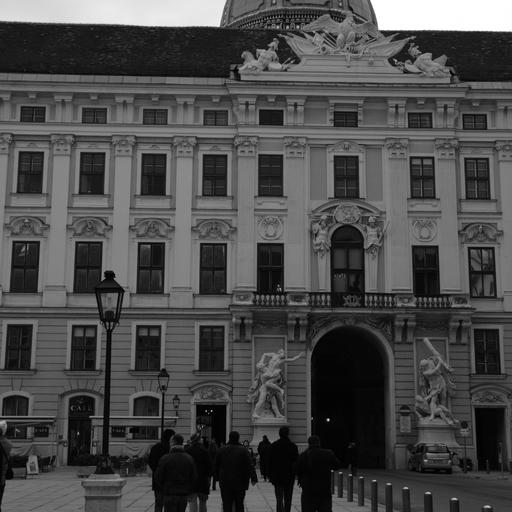
\includegraphics[scale=0.3]{13}
%        \caption{Image from BOSS base}
%    \end{figure}
%\end{frame}
    
%\begin{frame}{Probability map}
%    \begin{figure}[h]
%        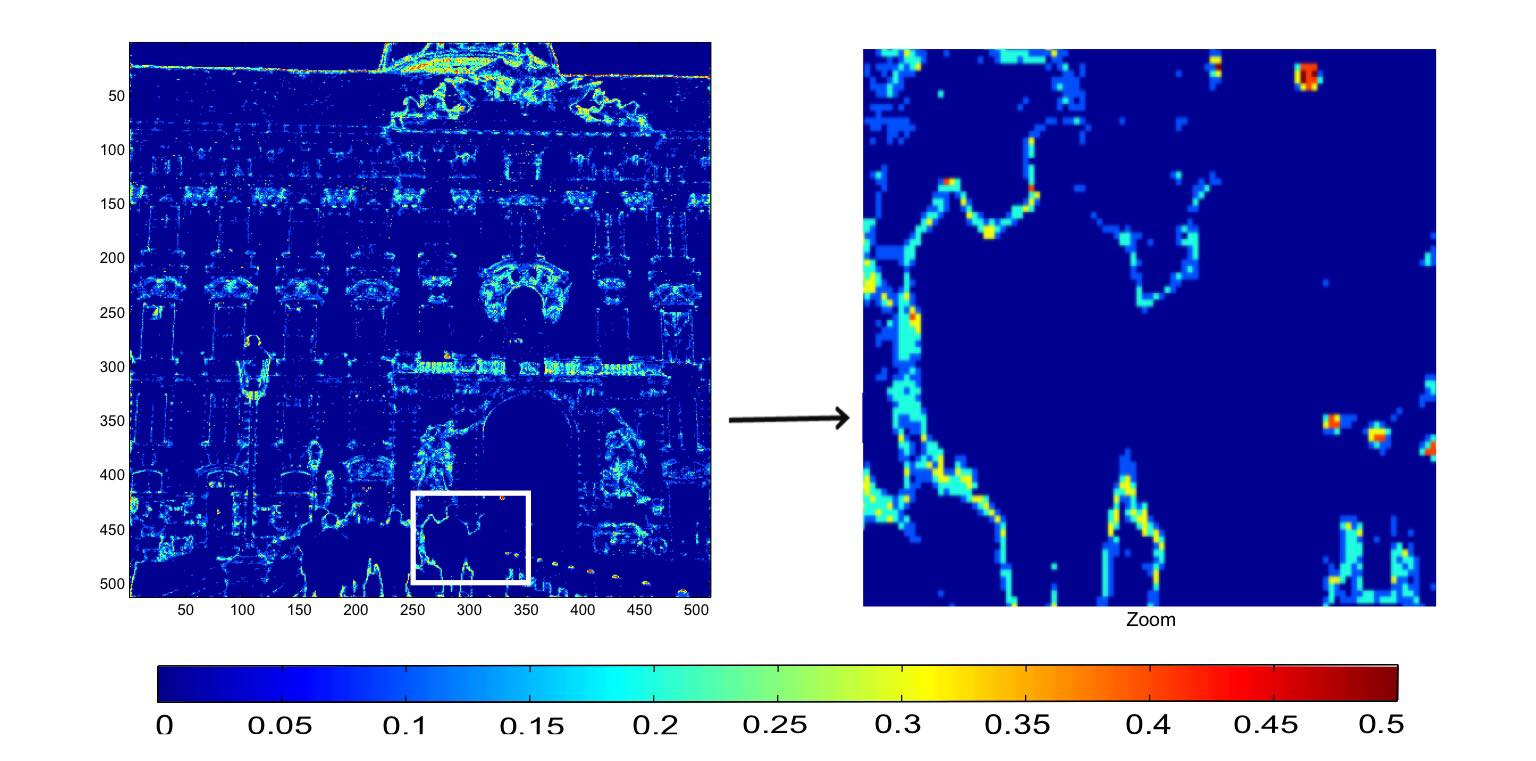
\includegraphics[scale=0.2]{probabilities}
%        \caption{Probability map of embedding for the same image when HUGO steganographic scheme is used at 0.2 bpp}
%    \end{figure}
%\end{frame}


\section*{Steganalysis}

\begin{frame}{Steganalysis}

    \begin{center}
        \alert{Detecting the presence of a message in an image.}
    \end{center}

    \pause
    Historically (until 2015): via features extraction followed by classification, for example histogram attacks~\only<2>{\footfullcite{fridrich2001detecting}}.
    \begin{figure}
        \includegraphics[width=0.9\linewidth]{histograms.pdf}
    \end{figure}

\end{frame}


\begin{frame}{Machine learning - Parameters, loss and optimization}
    \pause

    \begin{itemize}
        \setlength\itemsep{2em}

        \item \alert{Parameters}: $f$ a function parametrized by parameters $\theta = \{\mathbf{w}, b \}$, for example:
            \begin{equation}
                f(\mathbf{x}) = \mathbf{x} \star \mathbf{w} + b
            \end{equation}
            with $\star$ the convolution operation.

        \pause
        \item \alert{Loss}: $L$ a loss function giving the correctness of the classifier w.r.t true labels.

        \pause
        \item \alert{Optimization}: $f$ optimized via gradient descent with $\grad_\theta f$, via \textbf{backpropagation}.
                
    \end{itemize}

\end{frame}


\begin{frame}{Machine learning for automatic binary classification}
    %\animategraphics[width=0.9\linewidth]{25}{animation_training/}{0}{30}
\end{frame}


\begin{frame}{Steganalysis}

    Since 2015: \alert{Convolution Neural Networks (CNN)}. 

    \begin{tabular}{p{0.5\linewidth}p{0.5\linewidth}}
        
        Classifier $f$, where $f : \mathcal{I} \rightarrow [0,1]$.

        \begin{equation*}
            \left\{
            \begin{array}{ll}
            \mbox{If } f(\mathbf{x}) < 0.5 & \mbox{ then } \mathbf{x}\mbox{ classified as cover} \\
            \mbox{If } f(\mathbf{x}) \geq 0.5 & \mbox{ then } \mathbf{x}\mbox{ classified as stego} \\
            \end{array}
            \right.
        \end{equation*}

        \pause
        & Sate-of-the-art of architectures:
        \begin{itemize}
            \item XU-Net~\only<2>{\footfullcite{xu2017deep}},
            %\item Ye-Net~
            \item SRNet~\only<2>{\footfullcite{boroumand2018deep}},
            \item Efficient-Net~\only<2>{\footfullcite{tan2019efficientnet}}.
        \end{itemize}

    \end{tabular}

\end{frame}



\begin{frame}{Adversarial steganography}
    
    \begin{figure}
        \includegraphics[width=0.6\linewidth]{pingpong.pdf}
    \end{figure}

    \begin{center}
        \begin{itemize}
            \item $\mathcal{A}_{\text{alice}}$: set of actions of Alice
            \item $\mathcal{A}_{\text{eve}}$: set of actions of Eve
        \end{itemize}
    \end{center}

\end{frame}

\begin{frame}{Adversarial steganography}
    %\animategraphics[width=0.9\linewidth]{25}{animation_adversarial_stego/}{0}{30}
\end{frame}


\begin{frame}{Adversarial steganography}
    %\animategraphics[width=0.9\linewidth]{25}{animation_retraining_stega/}{0}{30}
\end{frame}


\begin{frame}{The problem we tackle}

    %\centering{\alert{\Large{How to optimize cost maps w.r.t. a set of steganalysts?}}}
    %\centering{\alert{\Large{Can we use adversarial examples to improve steganography w.r.t a class of steganalysts?}}}

    \centering{\alert{\Large{1.How to iterate?}}} \\

    \centering{\alert{\Large{2.How to properly achieve adversarial steganography?}}}

    %\pause
    %\vspace{2em}
    %\alert{Kerckhoffs’s principle}: Eve knows everything about Alice's strategy, except the secret key.
    
\end{frame}


% \begin{frame}{Adversarial steganography}

% Pingpong, cat-and-mouse game.
% Automatic game
% Loop between Alice and Eve

% Connection with Andrew and MiPod

% Adversarial example: ADV-EMB
% \minmax
    
% \end{frame}


\begin{frame}{Table of contents}
    \setbeamertemplate{section in toc}[sections numbered]
    \tableofcontents[hideallsubsections]
\end{frame}



\section{Playing an iterative game with a \textbf{minmax} protocol}




\begin{frame}{Past applications of game theory}

    \begin{itemize}
        %\item  Paper~\footfullcite{ker2016rethinking} shows for an aware steganalyst of the costs,  minimizing $\sum_{i,j} \pi_i^j \rho_i^j$ is \textit{naive}. The steganographer should play the minmax and equilibrium strategy: instead minimizing $\sum_{i, j, k} \pi_{i}^{j} c_{i}^{j, k} \pi_{i}^{k}$.
        \item Paper~\footfullcite{schottle2015game}
        \item Paper~\footfullcite{ker2016rethinking} proposes to solve the minmax and equilibrium strategy, when the steganalyst is aware of the cost map. But stays in a theoretical context.
    \end{itemize}
    
\end{frame}






\begin{frame}{Players with antagonists roles}

    \begin{tcolorbox}[colback=lightgreen,colframe=greentheme,title=\textbf{Definition} (Eve's utility)]
        For $(\mathcal{Y}, f)  \in \mathcal{A}_a \times \mathcal{A}_e$, Eve's utility is the accuracy of classification of $f$ between $\mathcal{X}$ and $\mathcal{Y}$, ie:
            \begin{equation}
                u_e(\mathcal{Y}, f) = \frac{1}{2} \left(\mathbb{E}_{\mathbf{x}\sim P_{\mathcal{X}}}[f(\mathbf{x}) < 0.5] + \mathbb{E}_{\mathbf{y} \sim \mathcal{Y}}[f(\mathbf{y})_ \geq 0.5] \right)
            \end{equation}
    \end{tcolorbox}

    \pause
    \begin{tcolorbox}[colback=lightgreen,colframe=greentheme,title=\textbf{Definition} (Alice's utility)]
        For $(\mathcal{Y}, f)  \in \mathcal{A}_a \times \mathcal{A}_e$, Alice's utility is equal to the opposite of Eve's utility:
            \begin{equation}
                u_a(\mathcal{Y}, f) = - u_e(\mathcal{Y}, f)
            \end{equation}
    \end{tcolorbox}

\end{frame}


\begin{frame}{Game theory expression of the problem}

    Solution concept:
    \alert{
        \Large{
            \begin{equation*}
            \underset{\mathcal{A}_a}{\argmin} \max_{\mathcal{A}_e} u_e(\mathcal{Y}, f)
            \end{equation*}
        }
    }

    \pause
    Solution approximated via a \alert{double oracle}~\only<2>{\footfullcite{adam2021double}} algorithm.
    
\end{frame}

    
\begin{frame}{Approximation with an iterative game}
    \begin{figure}
        \only<1>{\includegraphics[width=0.7\linewidth]{increasing_game_0.pdf}}
        \only<2>{\includegraphics[width=0.7\linewidth]{increasing_game_1.pdf}}
        \only<3>{\includegraphics[width=0.7\linewidth]{increasing_game_1_bis.pdf}}
        \only<4>{\includegraphics[width=0.7\linewidth]{increasing_game_2.pdf}}
        \only<5>{\includegraphics[width=0.7\linewidth]{increasing_game_2_bis.pdf}}
        \only<6>{\includegraphics[width=0.7\linewidth]{increasing_game_3.pdf}}
        \only<7>{\includegraphics[width=0.7\linewidth]{increasing_game_4.pdf}}
        \only<8>{\includegraphics[width=0.7\linewidth]{increasing_game_5.pdf}}
    \end{figure}
\end{frame}


% \begin{frame}{The $\min\max$ protocol}
% Approximating Alice's solution by: 

% \begin{enumerate}
%     \item \alert{adaptating the cost map}
% \begin{equation*}
% \begin{array}{ccccccccccc}
%     \mathbf{x} & \longrightarrow & \alert{\{\rho^b_i\}_i} & \longrightarrow & \{\pi_i^b\}_i &   \xrightarrow{\mbox{\footnotesize{draw}}} & \{b_i\}_i &  \longrightarrow & \mathbf{y} &  \longrightarrow & f(\mathbf{y})
% \end{array}
% \end{equation*}
    
% \pause

%     \item \alert{an iterative game at the image level}
    
% \begin{equation*}
%     \argmin_{\mathbf{y}} \max_{f\in\fset^k} f(\mathbf{y})
% \end{equation*}

% \end{enumerate}
% \end{frame}

\begin{frame}{The $\min\max$ protocol}
    \alert{Initialization}: $\mathcal{A}_e = \fset^{0} = \{f^0\}$,  $\mathcal{A}_a = \{\mathcal{Y}^0\}$. \\
    \pause
    \alert{At~$k^{\mathrm{th}}$ iteration}, the two following macro-steps: 
    \begin{enumerate}
        \item \alert<2>{Alice's turn.} 
            \begin{equation}
                \mathbf{y}^\ast = \arg \min_{\mathbf{y} \in \mathcal{A}_a} \max_{f \in \fset^{k-1}} f(\mathbf{y}).
                \label{eq:stepone}	
            \end{equation}
            \pause
        \item Eve's turn. \\ Creation of a new detector $f^k$ and appends it to the pool $\fset^{k-1}$, i.e. $\fset^k = \fset^{k-1} \cup \{f^k\}.$
    \end{enumerate}
\end{frame}

% \begin{frame}{2. Eve's turn: iteration $k$}
% \pause
% A huge challenge of steganography comes from the knowledge of each player's action. 
% What assumes Alice can differ from the real actions of Eve. 
% \pause
% $$ \mathcal{A}_e \neq \tilde{\mathcal{A}}_e $$
% \end{frame}


\begin{frame}{Details of player's actions}

    \begin{enumerate}

        \item \alert{Alice's new action:}
            \begin{equation*}
                \begin{array}{ccccccccccc}
                    \mathbf{x} & \longrightarrow & \{\rho_i\}_i & \longrightarrow & \{\pi_i^b\}_i &   \xrightarrow{\mbox{\footnotesize{draw}}} & \{b_i\}_i &  \longrightarrow & \mathbf{y} & \longrightarrow  & f(\mathbf{y}) \\
                    & & & & & & & & & \alert{\xleftarrow{ \nabla_{\mathbf{y}} f(\mathbf{y}) }} 
                \end{array}    
            \end{equation*}

        ADV-EMB~\footfullcite{tang2019cnn} proposes the following update rule, with $\alpha=2$:
        \begin{equation}
            \rho_{i}^{+, new} = 
            \left\{
                \begin{array}{ll}
                    \rho_{i}^+/\alpha & \mbox{if } \frac{\partial f}{\partial y_{i}}\left(\mathbf{y}\right) < 0, \\
                    \rho_{i}^+ & \mbox{if } \frac{\partial f}{\partial y_{i}}\left(\mathbf{y}\right) = 0, \\
                    \rho_{i}^+ \alpha & \mbox{if } \frac{\partial f}{\partial y_{i}}\left(\mathbf{y}\right) > 0.
                \end{array}
            \right.
            \label{eq:qplus}
        \end{equation}

        \pause
        \item \alert{Eve's new action:} training of a new classifier $f^k$ to discriminate between $\mathcal{X}$ and $\mathcal{Y}^k$.

    \end{enumerate}

\end{frame}







% \begin{frame}{1. Alice's turn}
% ADV-EMB can be used to solve equation~(\ref{eq:stepone}). 
% X
% It is achevied by computing the set $$\{\arg \min_{\mathbf{z} \in \mathcal{A}_a} f^k(\mathbf{z})\}_k$$ 
% and then computing 
% $$y = \arg \min_{\mathbf{z} \in \mathcal{A}_a} \max_k f^k(\mathbf{z})$$
% \end{frame}


\begin{frame}{Results - How to read the plots }
    \begin{figure}
        \includegraphics[width=0.7\linewidth]{results3.pdf}
    \end{figure}
\end{frame}

\begin{frame}{Results - Experimental setup}
    
    Mismatch between what assumes Alice can differ from the real actions of Eve. 
    \begin{equation*}
        \begin{array}{ccc}
            \underbrace{\mathcal{A}_{\text{eve}}}_{\mbox{Assumed Eve's actions}} & \neq & \underbrace{\tilde{\mathcal{A}}_{\text{eve}}}_{\mbox{Real Eve's actions}} \\
            \pause \alert{\mbox{Targeted models}} & & \alert{\mbox{Blind models}}
        \end{array}
    \end{equation*}
    
    \pause
    Comparison of different strategies: 
    \begin{itemize}
        \item  Minmax: $\mathbf{y}^\ast = \arg \min_{\mathbf{y} \in \mathcal{A}_a} \max_{f \in \fset^{k-1}} f(\mathbf{y})$;
        \item  Last iteration: $\mathbf{y}^\ast = \arg \min_{\mathbf{y} \in \mathcal{A}_a}  f^{k-1}(\mathbf{y})$;
        \item  Random: $\mathbf{y}^\ast = \arg \min_{\mathbf{y} \in \mathcal{A}_a}  f^i(\mathbf{y})$ for $i\sim U(\{0,\dots,k-1\})$. 
    \end{itemize}

\end{frame}


\begin{frame}{Results - Comparison of strategies for JPEG at QF 75 and different payloads (bpnzAC)}
    \begin{figure}
        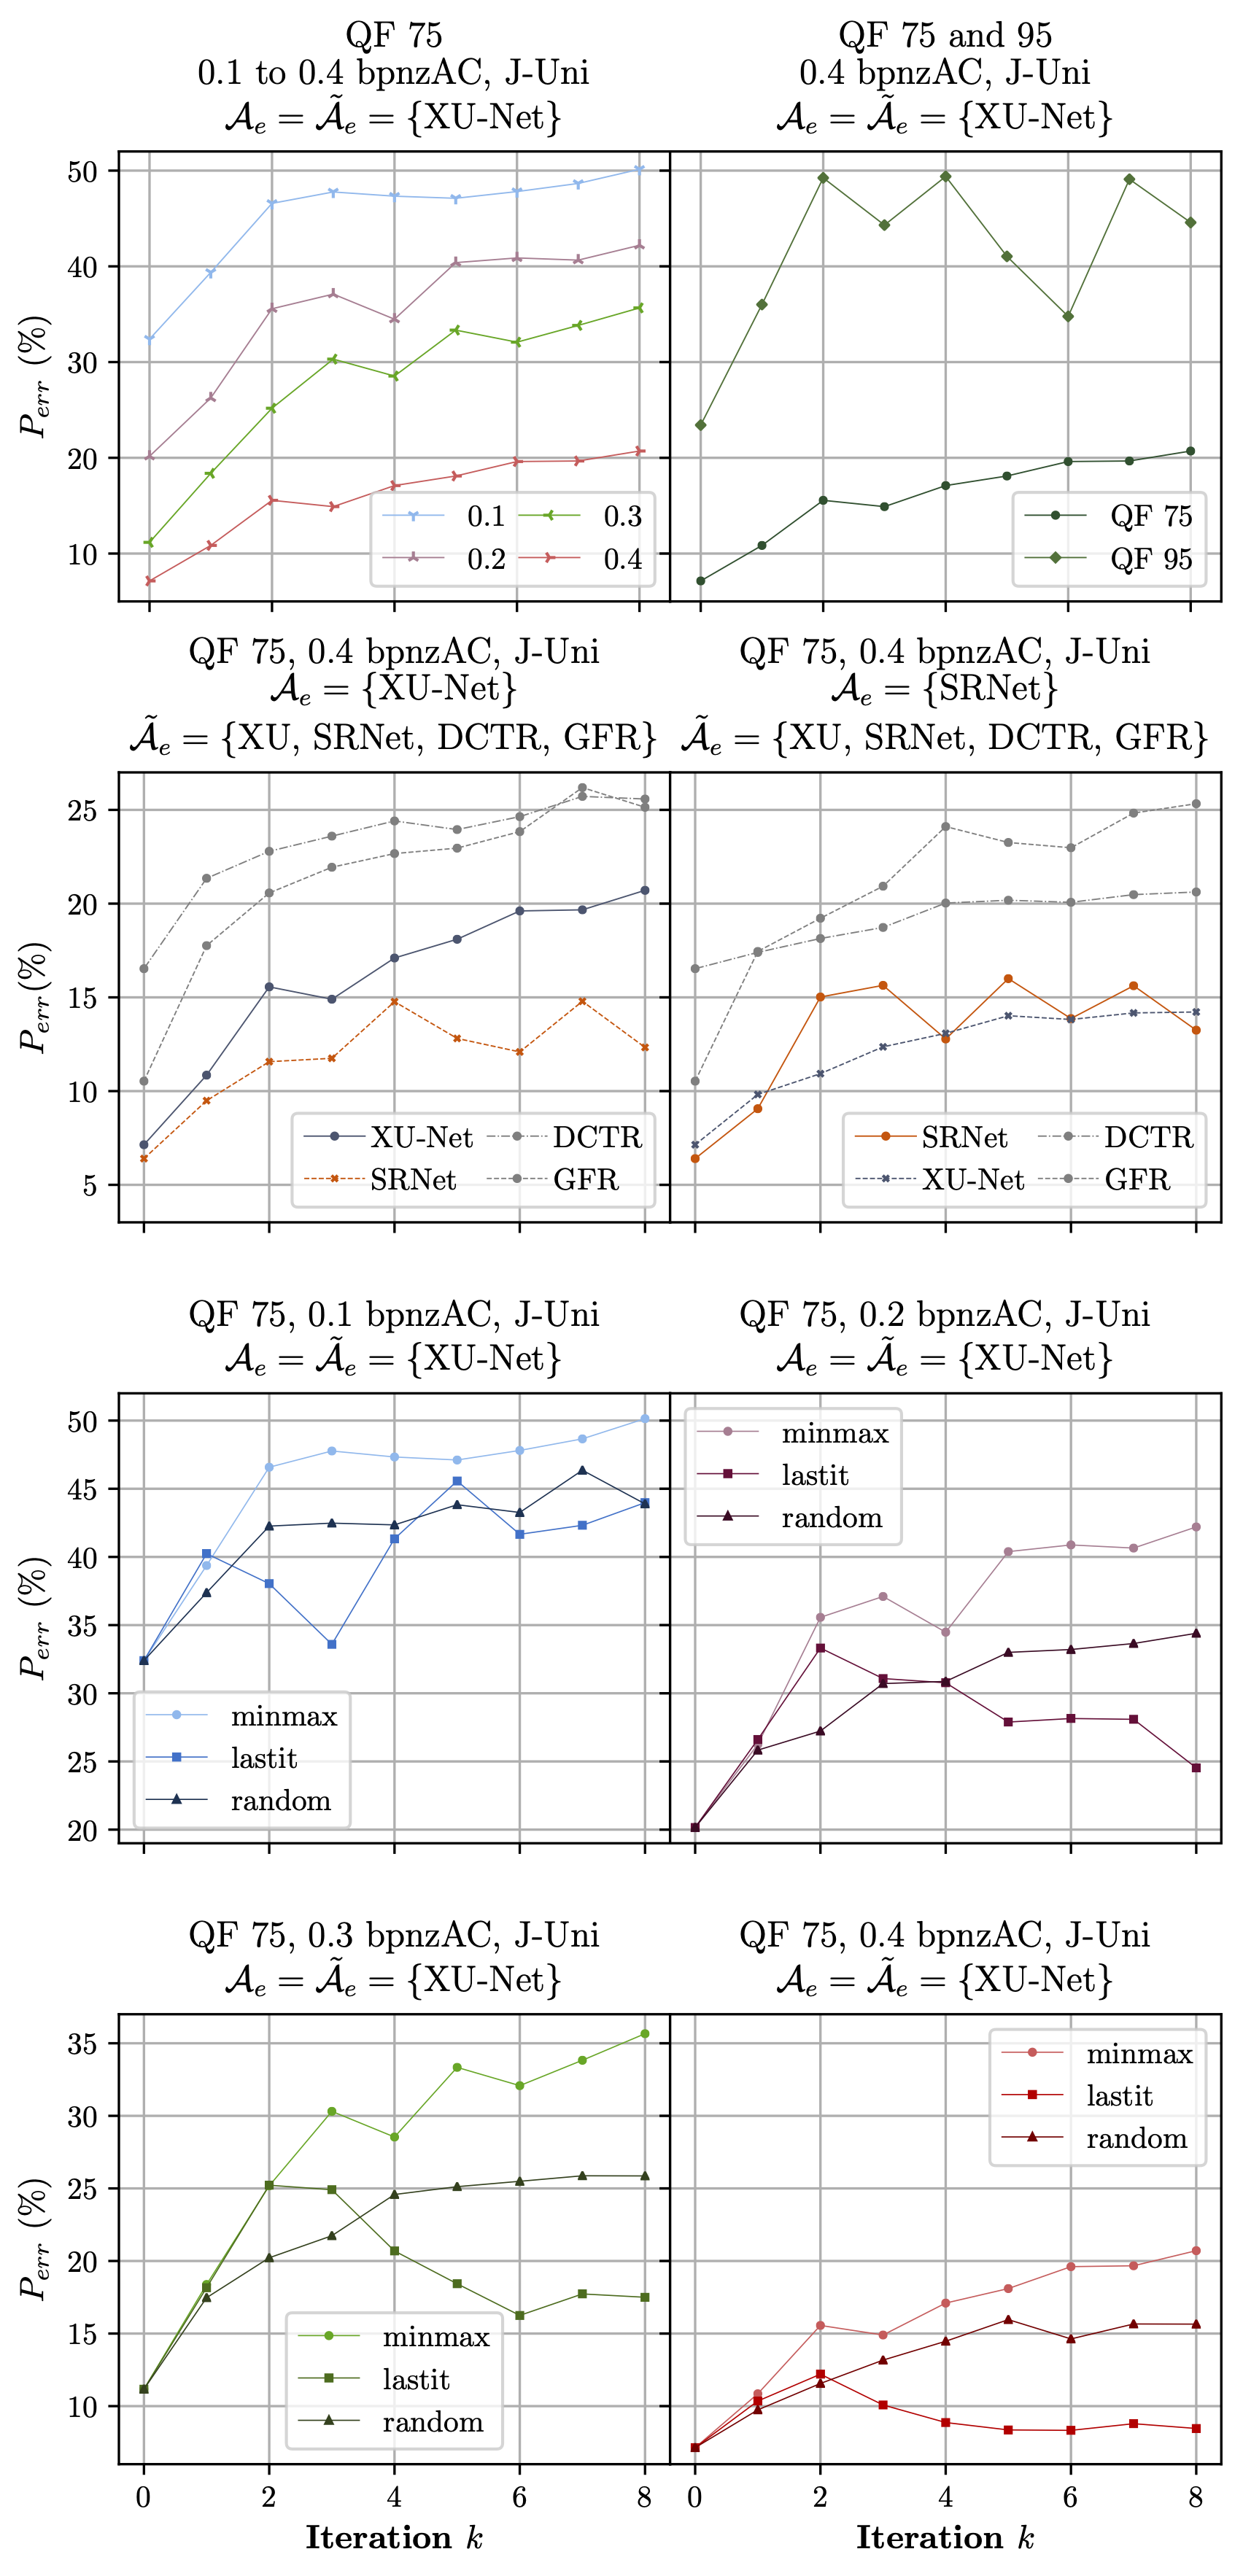
\includegraphics[width=0.8\linewidth]{minmax_prot_1.pdf}
        \includegraphics[width=0.8\linewidth]{abcisses.pdf}
    \end{figure}
\end{frame}

\begin{frame}{Results - Comparison of strategies for JPEG at QF 75 and different payloads (bpnzAC)}
    \begin{figure}
        \includegraphics[width=0.8\linewidth]{minmax_prot_2.pdf}
        \includegraphics[width=0.8\linewidth]{abcisses.pdf}
    \end{figure}
\end{frame}

\begin{frame}{Results - With different adversaries for JPEG QF 75, payload 0.4 bpnzAC}
    \begin{figure}
        \includegraphics[width=0.8\linewidth]{minmax_prot_3.pdf}
        \includegraphics[width=0.8\linewidth]{abcisses.pdf}
    \end{figure}
\end{frame}


\begin{frame}{Flaws of ADV-EMB}

    \begin{itemize}

        \item Heuristic
        
            \begin{equation}
                \rho_{i}^{+, new} = 
                \left\{
                    \begin{array}{ll}
                        \rho_{i}^+/\alpha & \mbox{if } \frac{\partial f}{\partial y_{i}}\left(\mathbf{y}\right) < 0, \\
                        \rho_{i}^+ & \mbox{if } \frac{\partial f}{\partial y_{i}}\left(\mathbf{y}\right) = 0, \\
                        \rho_{i}^+ \alpha & \mbox{if } \frac{\partial f}{\partial y_{i}}\left(\mathbf{y}\right) > 0,
                    \end{array}
                \right.
                \quad \mbox{with } \alpha = 2
            \end{equation}

    \end{itemize}

\end{frame}



\begin{frame}{Flaws of ADV-EMB}

    \begin{itemize}
            
        \item At some point, it fails at solving
            \begin{equation*}
                \mathbf{z}^\ast = \arg \min_{\mathbf{z} \in \mathcal{A}_a} \max_{f \in \fset^{k-1}} f(z).
            \end{equation*} 
            
            \begin{figure}
                \includegraphics[width=0.85\linewidth]{minmax_evolution_it9.pdf}
             \end{figure}
            
            \vspace{-0.7cm} \hspace{2cm}
            \begin{tabular}{m{5cm} m{2cm} m{4cm}}
                \hspace{2.2cm} $\mathbb{E}[f^k(\mathbf{z}_i)]$ & 
                $\mathbb{E}[\max_k f^k(\mathbf{z}_i)]$ &
                $\mathbb{E}[\arg \min_i \max_k f^k(\mathbf{z}_i)]$
            \end{tabular}
              
    \end{itemize}

\end{frame}
    



\section{Improving the cost map via a back-propagable attack: Backpack}


\begin{frame}{Backpack}

    \alert{Backpack}: \alert{Back-p}ropagable att\alert{ack} \pause in order to compute \alert{$\nabla_\rho \mathbb{E}_{y} [f(\mathbf{y})]$}.

    \begin{equation*}
        \begin{array}{ccccccccccc}
            \mathbf{x} \longrightarrow \{\rho_i\}_i & \longrightarrow  \{\pi_i^b\}_i    \xrightarrow{\mbox{\footnotesize{draw}}}  \{b_i\}_i   \longrightarrow  \mathbf{y}  \longrightarrow  & \mathbb{E}_{y} [f(\mathbf{y})] \\ 
            & \alert{\xleftarrow{\hspace{5em} \nabla_\rho \mathbb{E}_{y} [f(\mathbf{y})]\hspace{5em}}} 
        \end{array}
    \end{equation*}
    
    \pause
    For the chain rule, we need:
    \begin{equation*}
        \begin{array}{ccccccccccc}
            \mathbf{x} & \longrightarrow & \{\rho_i\}_i & \longrightarrow & \{\pi_i^b\}_i & \xrightarrow{\mbox{\footnotesize{draw}}} &  \{b_i\}_i  & \longrightarrow  & \mathbf{y} & \longrightarrow  & \mathbb{E}_{y} [f(\mathbf{y})] \\ 
            &&& \textcolor{greentheme}{\xleftarrow{\frac{\partial \pi}{\partial \rho} }}
            && \textcolor{greentheme}{\xleftarrow{\frac{\partial b}{\partial \pi} }}
            && \textcolor{greentheme}{\xleftarrow{\frac{\partial y}{\partial b}}}
            && \alert{\xleftarrow{\nabla_y \mathbb{E}_{y} [f(\mathbf{y})]}} 
            

        \end{array}
    \end{equation*}

    \pause
    \begin{equation*}
        \begin{array}{ccccccccccc}
            \mathbf{x} & \longrightarrow & \{\rho_i\}_i & \longrightarrow & \{\pi_i^b\}_i & \xrightarrow{\mbox{\footnotesize{draw}}} &  \{b_i\}_i  & \longrightarrow  & \mathbf{y} & \longrightarrow  & \mathbb{E}_{y} [f(\mathbf{y})] \\ 
            &&& \textcolor{orangetheme}{\xleftarrow{2. \frac{\partial \pi}{\partial \rho} }}
            && \textcolor{orangetheme}{\xleftarrow{1. \frac{\partial b}{\partial \pi} }}
            && \textcolor{greentheme}{\xleftarrow{\frac{\partial y}{\partial b}}}
            && \alert{\xleftarrow{\nabla_y \mathbb{E}_{y} [f(\mathbf{y})]}} 
        \end{array}
    \end{equation*}
    
    % \pause
    % \begin{enumerate}
    %     \item Approximation of discrete modification by continuous modifications controlled by a temperature $\tau$ 
    %         \begin{equation*}
    %             \begin{array}{ccccccccccc}
    %                 \mathbf{x} \longrightarrow \{\rho_i\}_i \longrightarrow  \{\pi_i^b\}_i    \alert{\xrightarrow{B} } \{\tilde{b}_i\}_i   \longrightarrow  \tilde{\mathbf{y}}  \longrightarrow  & \mathbb{E}[f(\tilde{\mathbf{y}})]
    %             \end{array}
    %         \end{equation*}
    
    %     \pause
    %     \item Computation of the gradient thanks to the gradient of a function defined implicitly
    %         \begin{equation*}
    %             \begin{array}{ccccccccccc}
    %                 \mathbf{x} \longrightarrow \{\rho_i\}_i \alert{\longrightarrow}  \{\pi_i^b\}_i    \longrightarrow \{\tilde{b}_i\}_i \longrightarrow  \tilde{\mathbf{y}}  \longrightarrow  & \mathbb{E}[f(\tilde{\mathbf{y}}])
    %             \end{array}
    %         \end{equation*}
    % \end{enumerate}

\end{frame}


% \begin{frame}{1. Approximation of discrete modifications}
%     \pause 
%     How to draw from the following categorical distribution? 
%     \begin{table}[h]
%         \centering
%         \begin{tabular}{c||c|c|c}
%             b & -1  & 0 & 1   \\ \hline
%             p & p^{-1}  & p^0 & p^{+1}   \\
%         \end{tabular} 
%         \hspace{2em} with $p^{-1} + p^0 + p^{+1} = 1$
%         \label{tab:probalaw}
%     \end{table}
    
%     % Two solutions:
%     % \begin{table}[h]
%     %     \centering
%     %     \begin{tabular}{c|c}
%     %         $u \sim U(0,1)$ & $g^{-1},g^{0},g^{+1}  \sim G(0,1)$ \\
%     %         $b =\left\{
%     %             \begin{array}{ll}
%     %               -1 & \text{ if } u < p^{-1}\\
%     %               0 & \text{ elif } u < p^{-1}+p^0\\ 
%     %               +1 & \text{ else}
%     %             \end{array}
%     %           \right.$
             
%     %          & $b = \argmax_{j \in\{-1,0,1\}} g^{j} + \log p^j$
%     %     \end{tabular}
%     %   \label{tab:drawlaw}
%     % \end{table}
%     \pause
%     Possible solution: draw $g^{-1},g^{0},g^{+1}  \sim G(0,1)$, then
%     \begin{equation}
%         b = \argmax_{j \in\{-1,0,1\}} g^{j} + \log p^j
%     \end{equation}  \pause
    
%     \begin{equation}
%         \mbox{one-hot}\left(\argmax_{j \in\{-1,0,1\}} g^{j} + \log p^j\right) = \alert{\lim_{\tau \rightarrow 0} \softmax_{j \in\{-1,0,1\}}\left(\frac{g^{j} + \log p^j}{\tau}\right)}
%     \end{equation}

% \end{frame}

% \begin{frame}{1. Approximation of discrete modifications with Softmax Gumbel distribution}
%     \begin{equation}
%     \begin{aligned}
%     \nabla_{\bm{\rho}} \underset{\vec{b}\sim P_\vec{b}\left(\vec{b} | \bm{\rho}, \lambda\right)}{\mathbb{E}}\left[f\left(\vec{x}+\vec{b}\right)\right] = 
%     & \nabla_{\bm{\rho}} \underset{\vec{r} \sim R}{\mathbb{E}}[f(\vec{x}+B(\bm{\pi},\vec{r}))]  \\
%     &  = \underset{\vec{r} \sim R}{\mathbb{E}}\left[ \nabla_{\bm{\rho}}  f(\vec{x}+B(\bm{\pi},\vec{r}))\right] 
%     \label{eq:permutategradientexpectancy}
%     \end{aligned}
%     \end{equation}
% \end{frame}


\begin{frame}{1. Approximation of discrete modifications with Softmax Gumbel distribution}
    
    \begin{equation*}
        \begin{array}{ccccccccccc}
            \mathbf{x}&  \longrightarrow & \{\rho_i\}_i & \longrightarrow  & \{\pi_i^b\}_i  &   \alert{\xrightarrow{\mbox{\footnotesize{draw}}}}  & \{b_i\}_i  &  \longrightarrow  & \mathbf{y}  & \longrightarrow  & \mathbb{E}_{y} [f(\mathbf{y})] \\ 
            \pause & & & & & \textcolor{orangetheme}{\xleftarrow{\frac{\partial b_i }{\partial \pi_i^b} }}
        \end{array}
    \end{equation*}
    
    \pause
    Rewriting the \textit{drawing} step as the output of a deterministic function $B(\pi, u)$:
    \begin{equation*}
        \begin{array}{ccccccccccc}
            \mathbf{x} & \longrightarrow & \{\rho_i\}_i & \longrightarrow  & \{\pi_i^b\}_i  &  \alert{\xrightarrow{B(., u)} } & \{b_i\}_i  &  \longrightarrow  & \mathbf{y} & \longrightarrow  & \mathbb{E}[f(\mathbf{y})]
        \end{array}
    \end{equation*}

    \pause
    Smooth approximation of $B$ by $B_\tau$: 
    \begin{equation*}
        \begin{array}{ccccccccccc}
            \mathbf{x} & \longrightarrow & \{\rho_i\}_i & \longrightarrow &  \{\pi_i^b\}_i  & \alert{\xrightarrow{B_\tau(.,u)} } & \{\tilde{b}_i\}_i  & \longrightarrow  & \tilde{\mathbf{y}} & \longrightarrow  & \mathbb{E}[f(\tilde{\mathbf{y}})] \\
            \pause & & & & & \textcolor{greentheme}{\xleftarrow{\frac{\partial \tilde{b}_i }{\partial \pi_i^b} }}
        \end{array}
    \end{equation*}

\end{frame}


\begin{frame}{1. Approximation of discrete modifications with Softmax Gumbel distribution}

    \begin{tcolorbox}[colback=lightgreen,colframe=greentheme,title=\textbf{Definition} (Hardmax Gumbel Function)]
        Hardmax Gumbel\footnotemark~is a function of  $\pi = \{\pi^{-1},\pi^{0}, \pi^{+1}\}$ and $\vec{g} = \{g^{-1},g^{0}, g^{+1}\}$ and simulates, when $\vec{g}$ is drawn from $G(0,1)$ a drawing from a categorical distribution in $\{-1,0,1\}$ with probability distribution $\pi$:  
        \begin{equation}
            b = \mbox{HG}(\bm{\pi}, \vec{g}) = \underset{{j \in \{-1,0,+1\}}}{\arg \max} (g^j+ \log \pi^j).
        \end{equation}
    \end{tcolorbox}

    \footcitetext{jang2016categorical}

\end{frame}

\begin{frame}{1. Approximation of discrete modifications with Softmax Gumbel distribution}
    
    The softmax function, an approximation of $\argmax$ function:
    \begin{equation}
        \mbox{softmax}\left(z_1,\ldots,z_n\right) = \frac{1}{\sum_{k=1}^n e^{z_k}}(e^{z_1},\ldots,e^{z_n}),
    \end{equation}

    because: 
    \begin{equation}
        \lim_{\tau \rightarrow 0} \mbox{softmax}\left(\frac{z_1}{\tau},\ldots,\frac{z_n}{\tau}\right) = \underbrace{(0,0\ldots,0,1,0,\dots, 0)}_{1 \text{ at position } \arg \max \text{HG}}, 
    \end{equation}

    $\tau$ is called the \emph{temperature}.

\end{frame}

\begin{frame}{1. Approximation of discrete modifications with Softmax Gumbel distribution}
    
    \begin{tcolorbox}[colback=lightgreen,colframe=greentheme,title=\textbf{Definition} (Softmax Gumbel Function)]

        Hardmax Gumbel function can be approximated by the following Softmax Gumbel function: 
        \begin{eqnarray}\label{eq:softmaxgumbel} 
            \tilde{b}_{\tau} &=& \mbox{SG}_\tau(\bm{\pi}, \vec{g}) = \sum_{j \in \{-1,0,+1\}} j\;z^j,\\
            \text{with } \vec{z} &=& \mbox{softmax}\left(\frac{\vec{g}+\log \bm{\pi}}{\tau}\right).
        \end{eqnarray}

    \end{tcolorbox}

\end{frame}





\begin{frame}{1. Approximation of discrete modifications with Softmax Gumbel distribution}
    \begin{figure}[h]
        \includegraphics[width=0.8\linewidth]{ternarychanges_softmaxgumbel.pdf}
    \end{figure}
\end{frame}



\begin{frame}{2. $\frac{\partial \mathbf{\pi}}{\partial \rho}$ computed implicitly}
    \begin{equation*}
        \begin{array}{ccccccccccc}
            \mathbf{x} & \longrightarrow & \{\rho_i\}_i & \longrightarrow & \{\pi_i^b\}_i & \longrightarrow &  \{b_i\}_i  & \longrightarrow  & \mathbf{y} & \longrightarrow  & \mathbb{E}_{y} [f(\mathbf{y})] \\ 
            &&& \textcolor{orangetheme}{\xleftarrow{\frac{\partial \pi}{\partial \rho} }}
        \end{array}
    \end{equation*}

    \pause
    Probabilities are a function of costs $\rho$ and $\lambda$
    \begin{equation}
        \pi_i^j = P_i^j\left(\rho_{i}, \lambda\right) =\frac{e^{-\lambda \rho_{i}^{j}}}{\sum_{k \in \{-1,0,1\}} e^{-\lambda \rho_{i}^{k}}}, \quad j \in \{-1, 0, 1\}
    \end{equation}


    The chain rule gives:
    \begin{equation}
        \frac{d \bm{\pi}}{d \bm{\rho}} = \frac{\partial \bm{\pi}}{\partial \bm{\rho}} + \frac{\partial \bm{\pi}}{\partial \lambda} \textcolor{orangetheme}{\nabla_{\bm{\rho}} \lambda}
        \label{eq:gradientprobabilities}
    \end{equation}

    %\pause
    where $\lambda = \alert{\Lambda(\rho,|\mathbf{m}|))}$ is an (implicit) function of $\rho$ and $|m|$ stemming from the entropy constraint: 
    $ H(\boldsymbol{\pi})=|\mathbf{m}|$
   

\end{frame}

\begin{frame}{2. $\frac{\partial \mathbf{\pi}}{\partial \rho}$ computed implicitly}
    
    The total derivative of $H$: 
    \begin{equation}
        \nabla_{\boldsymbol{\rho}} H(\boldsymbol{\pi}) \frac{\partial \boldsymbol{\rho}}{\partial \boldsymbol{\rho}}+\frac{\partial H(\boldsymbol{\pi})}{\partial \lambda} \nabla_{\boldsymbol{\rho}} \lambda=0
    \end{equation}

    \pause
    Explicit gradient of $\lambda$ accessible through differentiation of the entropy constraint.
    \begin{equation}
        \nabla_{\bm{\rho}} \lambda =  -\left( \frac{\partial  H(\bm{\pi})}{\partial \lambda}\right)^{-1} \nabla_{\bm{\rho}} H (\bm{\pi}) .
    \end{equation}

\end{frame}


% \begin{frame}{2. $\frac{\partial \mathbf{p}}{\partial \rho}$ computed implicitly}

%     Full expression of the gradient :
%     \begin{equation}
%         \frac{\partial \mathbf{p}}{\partial \rho}=\frac{\partial P_{\mathbf{b}}}{\partial \rho} \frac{\partial \rho}{\partial \rho}+\frac{\partial P_{\mathbf{b}}}{\partial \lambda} \alert{\frac{\partial \Lambda(\rho,|\mathbf{m}|))}{\partial \rho}}
%     \end{equation} \pause
%     But because the condition on entropy:
    
%     \begin{equation}
%         H\left(P_{\mathbf{b}}(\lambda, \rho)\right)=H\left(P_{\mathbf{b}}(\Lambda(\rho,|\mathbf{m}|), \rho)\right)=|\mathbf{m}|
%     \end{equation} \pause
    
%     The derivative w.r.t. $\rho$ is equals to zero:
%     \begin{equation}
%         \frac{\partial H\left(P_{\mathbf{b}}\right)}{\partial \rho} \frac{\partial \rho}{\partial \rho}+\frac{\partial H\left(P_{\mathrm{b}}\right)}{\partial \lambda} \alert{\frac{\partial \Lambda}{\partial \rho}}=0
%     \end{equation}
% \end{frame}


\begin{frame}{Overall algorithm of Backpack}


    \alert{Backpack}: \alert{Back-p}ropagable att\alert{ack}.
    %    \begin{align*}
    %     \mathbf{x} \longrightarrow \rho_i \alert{\longrightarrow} \pi_i \alert{ \xrightarrow{\tilde{b}_\tau}} \tilde{\mathbf{y}} & \longrightarrow f(\tilde{\mathbf{y}}) %\\
    %     % & \longrightarrow f^1(\tilde{\mathbf{y}}) \\
    %     % & \dots \\
    %     % & \longrightarrow f^{k-1}(\tilde{\mathbf{y}})
    %     \end{align*}

    \begin{equation*}
        \begin{array}{ccc}
            \mathbf{x} \longrightarrow \{\rho_i\}_i & \alert{\longrightarrow}  \{\pi_i^b\}_i    \alert{\longrightarrow} \{\tilde{b}_i\}_i \longrightarrow  \tilde{\mathbf{y}}  \longrightarrow  & \mathbb{E}_{\tilde{y}}[f(\tilde{\mathbf{y}})] \\
            & \alert{\xleftarrow{\hspace{5em} \nabla_\rho \mathbb{E}_{\tilde{y}} [f(\tilde{\mathbf{y}})]\hspace{5em}}} 
        \end{array}
    \end{equation*}

    \pause
    Iterative gradient descent, while playing with the temperature $\tau$, to optimize the smooth output w.r.t. best detector:

    \begin{equation}
        \alert{\nabla_\rho \mathbb{E}_{\tilde{y}} [f(\tilde{\mathbf{y}})]}, \quad  f = \argmax_{f \in \mathcal{F}^{k-1}} \mathbb{E}_{\tilde{y}} [f(\tilde{\mathbf{y}})]
    \end{equation}

\end{frame}


\begin{frame}{Difference between smooth and discrete stegos}

    \begin{columns}[c] 
        \begin{column}{.65\textwidth}
            \begin{figure}[h]
                \includegraphics[width=1\textwidth]{gradient_descent_purpose_tau.pdf}
            \end{figure}
        \end{column}  
        
        \pause
        \begin{column}{.3\textwidth}
            Hyper-parameters:
            %\begin{minipage}[c][width=1\textwidth]
                \begin{itemize}
                    %\setlength\itemsep{2em}
                    \item Number of samples
                    \item Temperature policy
                    \item Number of steps for the gradient descent
                    \item Stopping condition (here depends on the value of the detectability of covers)
                \end{itemize}
            %\end{minipage}
        \end{column}  
    \end{columns}

\end{frame}


% \begin{frame}{Overall algorithm: hyperparameters}
% Hyperparameters:
%     \begin{itemize}
%         \item \alert<1>{Learning rate and optimizer} $\quad \alpha=5e^{-2}$ or $\alpha=5e^{-1}$ with ADAM. \pause
%         \item \alert<2>{Starting temperature $\tau_0$. }  $ \quad  \tau_0 = 1$. \pause
%         \item \alert<3>{When to decrease the temperature.} $\quad \max_f |f(\tilde{\mathbf{y}}) - f(\mathbf{x})| < \epsilon$. \pause
%         \item \alert<4>{How to decrease the temperature.} $\quad  \tau \leftarrow \tau/2$ \pause
%         \item \alert<5>{Stopping condition.} $\quad \max_f |f(\mathbf{y}) - f(\mathbf{x})| < \epsilon$. \pause
%         \item \alert<6>{Maximum number of steps.} 
%     \end{itemize}
% \end{frame}



\begin{frame}{Evolution of $\min\max$ protocol with ADV-EMB}
    \begin{figure}
        \includegraphics[width=0.9\linewidth]{minmax_evolution_it9.pdf}
    \end{figure}
\end{frame}


\begin{frame}{Evolution of $\min\max$ protocol with Backpack}
    \begin{figure}
        \includegraphics[width=0.9\linewidth]{minmax_SGE_evolution_it7.pdf}
    \end{figure}
\end{frame}



\begin{frame}{Results - Comparison ADV-EMB and Backpack for JPEG at QF 75 and at payload 0.4 bpnzAC}
    \begin{figure}[h]
        \includegraphics[width=\linewidth]{pe_protocol_comparison_75.pdf}
    \end{figure}
\end{frame}


\begin{frame}{Results - With three targeted models, for images at QF 75 and payload 0.4 bpnzAC}

    \begin{figure}[h]
        \includegraphics[width=0.55\linewidth]{QF75_3models.pdf}
    \end{figure}
    \pause
    \begin{center}
        \begin{tabular}{ccccc}
           \textbf{EfNet} & \textbf{XU-Net} & \textbf{SRNet} & DCTR & GFR \\
           \alert{$+31.6 $ pts} & \alert{$+31.0$ pts} & \alert{$+38.2 $ pts} & $+20.5$ pts & $+27.0 $ pts
        \end{tabular}
    \end{center}
    
\end{frame}


\begin{frame}{Results - Protocol with Backpack, at QF 100, with e-XUNet}
Classifier using the rounding error of decompression~\footfullcite{butora2019reverse}
    \begin{figure}[h]
        \includegraphics[width=0.5\linewidth]{experience_512_100_0_01_SGE_exunet.pdf}
    \end{figure}
\end{frame}


\begin{frame}{Interpretation - Natural correlations between DCT modes~\footfullcite{taburet2019computing}}
    \begin{tabularx}{0.9\textwidth} { 
        >{\centering\arraybackslash}X 
        >{\centering\arraybackslash}X 
        >{\centering\arraybackslash}X
        >{\centering\arraybackslash}X  }
        Intra-block & Inter-block & Inter-block & Inter-block \\ 
        &  $\rightarrow$ & $\downarrow$& $\searrow$ 
   \end{tabularx}

    \begin{figure}[h]
        \includegraphics[width=1\linewidth]{cov_BOSS.pdf}
    \end{figure}
\end{frame}


\begin{frame}{Interpretation - Observed correlations between changes of DCT modes}
    % \begin{center}
    %         \begin{tabular}{| m{5em} | m{1cm}| m{1cm} |}
    %         Intra-block & Inter-block & Inter-block & Inter-block \\ 
    %         \end{tabular}
        
    % \end{center}

    \begin{tabularx}{0.9\textwidth} { 
         >{\centering\arraybackslash}X 
         >{\centering\arraybackslash}X 
         >{\centering\arraybackslash}X
         >{\centering\arraybackslash}X  }
         Intra-block & Inter-block & Inter-block & Inter-block \\ 
         &  $\rightarrow$ & $\downarrow$& $\searrow$ 
    \end{tabularx}

    \begin{figure}[h]
        \includegraphics[width=1\linewidth]{covariance_QF100_0_01_firstline.pdf}
    \end{figure}

    \pause
    For symmetric costs, correlations between DCT modes are equal to 0. 
    
\end{frame}




\section{Conclusion and perspectives}


\begin{frame}{Conclusion}

    \begin{itemize}
        \item First contribution~\footfullcite{bernard2020explicit}: Automatic game between Alice and Eve. 
        
            \begin{columns}[c] 
                \begin{column}{.5\textwidth}
                    \begin{figure}[h]
                        \includegraphics[width=0.30\linewidth]{historicalgraph.pdf}
                    \end{figure}
                \end{column}  
                
                \pause
                \begin{column}{.5\textwidth}
                    \begin{figure}[h]
                        \includegraphics[width=1\linewidth]{pingpong.pdf}
                    \end{figure}
                \end{column}  
            \end{columns}
        
    \end{itemize}
\end{frame}


\begin{frame}{Conclusion}

        \begin{itemize}
            %\setlength\itemsep{2em}
            \item Design of a new attack~\footfullcite{bernard2020explicit} to optimize a cost map w.r.t. a set of classifiers
            \pause     
            \begin{figure}[h]
                    \includegraphics[width=0.4\textwidth]{pingpong_backpack.pdf}
                \end{figure}
            \item Notable improvement
            \item Reproducibility: available on Gitlab \url{https://gitlab.univ-lille.fr/solene.bernard/backpack}
        \end{itemize}  

\end{frame}


\begin{frame}{Perspectives}

    \begin{itemize}

        \item Backpack very computationnaly costly, and gets worst with increasing iterations of the protocol. 
        
        \begin{figure}[h]
            \includegraphics[width=0.4\linewidth]{experience_512_100_0_01_SGE_exunet.pdf}
        \end{figure}

        \pause

        \begin{itemize}
            \item Distillation: to merge the knowledge of multiple classifiers
            %\item Attacking a random subset of classifier
            \item Hyper-parameters to optimize for Backpack: number maximum of steps, learning rate, stopping condition.
        \end{itemize}

    \end{itemize}

\end{frame}

\begin{frame}{Perspectives}
    Experiment at payload \alert{0.4 bpnzAC} with targeted XUNet, SRNet, and Efficient-Net.
    \begin{figure}[h]
        \includegraphics[width=1\linewidth]{mismatch_payload.pdf}
    \end{figure}
    
    \begin{itemize}
        \item Payload dependent: specific to the payload
            \begin{itemize}
                \item diversify the payload
            \end{itemize}
    \end{itemize}

\end{frame}



\begin{frame}{Perspectives}
  
    \begin{itemize}
        \setlength\itemsep{2em}
    
        \item Source dependent: the whole protocol should be re-run for every cover source,  
                
            \begin{itemize}
                \item diversify the cover source
            \end{itemize}
            
        \pause 
        
        \item Improving the $\min\max$ strategy by considering mixed strategies
            \begin{itemize}
                \item Consider strategy profiles which are a distribution over the set of actions
            \end{itemize}

        \item Considering embedding changes with bigger amplitude (not only ternary embedding)
            \begin{itemize}
                \item quinary, septenary...
            \end{itemize}

        %\item Change float precision for the computation of the gradient
    
    \end{itemize}

\end{frame}


%\bibliographystyle{acm}
%\bibliography{demo}

\end{document}
